\vspace{10pt}

{\centering\subsection*{周曼读:清贫有感}}

\addcontentsline{toc}{subsection}{周曼读:清贫有感}

\renewcommand{\leftmark}{周曼读:清贫有感}

\begin{figure}[htbp]

\centering

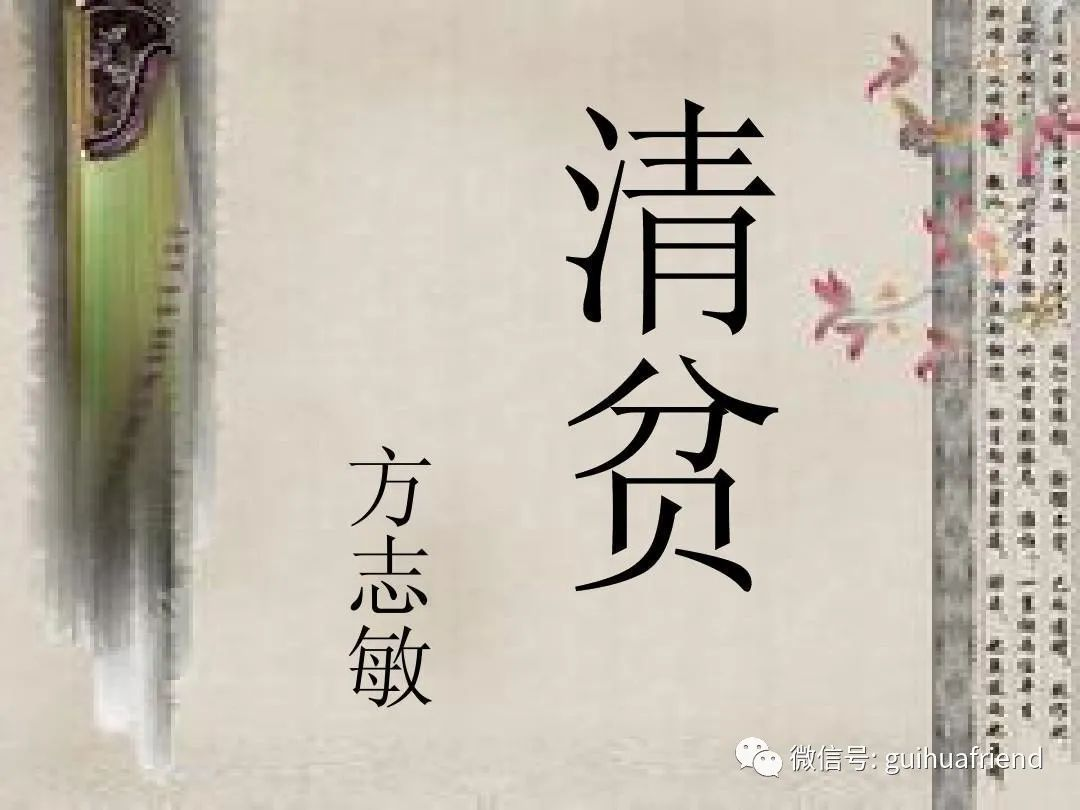
\includegraphics[width = .5\textwidth]{./ch/36.jpg}

\end{figure}



或许你要问我为什么会喜欢《清贫》这篇文章,那就让我自豪的告诉你吧!



我最喜欢《清贫》里的一句话,“你们要相信我说的话,不要瞎忙吧,我不比你们国民党当官,个个都有钱,我今天确实一个铜板都没有,我们革命不是为了发财!”这里写方志敏同志向两个国民党士兵解释他确实没有钱。而且方志敏同志的回答字字有力,落地有声,赞扬了共产党人恪守清贫的美德。

清贫是一种不为物质生活所束缚的生活态度,是一种物质财富视而不见的生活状态。以方志敏同志为代表的革命者视清贫为德,以清贫为乐,并以此作为战胜困难的法宝。这是多么高尚的思想境界啊!

我觉得《清贫》这篇文章,展现出一位共产党人坚定的革命信念和矜持不苟、 舍己为公的高尚品质。

而且《清贫》这篇文章是写那些“富翁们”不理解革命者甘于清贫,矜持不苟,舍己为公的高尚情操,因为他们只会过奢侈腐败的生活。运用反语,讽刺了国民党官员贪婪,自私的恶习。方志敏同志的清贫、朴素是革命者战胜困难的力量的源泉。

这就是我喜欢清贫这篇文章的原因,我推荐你们去看哦!







\vspace{10pt}



作者:五(1)班 周曼



指导老师:李哲茜



投稿:2021年 4月21日



发表:2021年4月26日






                



\vspace{10pt}

\hline



